\newcommand{\archid}{1}
\chapter{Design of IoT platform architecture}
%What needs to be monitored: sensor-networks/IoT 
%How data and information streams flow and combine 
%will focus on data sources and streams as to ascertain which architecture, configuration and components are needed/suitable.
\section{Problem statement}
\subsection{Goal}
\subsection{Variety/commonlity analysis}
\subsubsection{Definitions}
\begin{description}
\nospace
\item[Platform:] the monitoring platform to be designed.
\item[Application:] the application that is being investigated by the platform.
\item[Snapshot:] a collection of data points indicating the state of a system on a certain  [point in time].
\item[Source:] a device (external) or process (internal).
\item[Consequence:] an action taken by the platform based on the analysis of one or more snapshots.
\end{description}
\subsubsection{Commonalities}
\begin{enumerate}[label=C\archid .\arabic*]
\nospace
\item transform snapshots
\end{enumerate}
\subsubsection{Variety}
%TODO iets over QoI and information real-estate/capacity
conclusion basis
\begin{enumerate}[label=V\archid .\arabic*]
\nospace
\item \label{v:basis_single} single snapshot. (e.g. )
\item \label{v:basis_historic} multiple temporally ordered snapshots from a single source. Used to analyse tendency of parameters. (e.g. )
\item \label{v:basis_accumulated} many snapshots multi-source without individual significance. (e.g. )
\end{enumerate}
We can never anticipate the exact consequence intended for a [certain] application.
\begin{enumerate}[label=V\archid .\arabic* , resume]
\nospace
\item \label{v:consequence_implementation} The possible consequences by the platform have a large range of implementations.
\end{enumerate}
Though the exact implementation of consequences can never be [exactly] anticipated, we can identify some [common] types for a consequence.
\begin{enumerate}[label=V\archid .\arabic* , resume]
\nospace
\item \label{v:consequence_general_reporting} build a model for general/global reports. Either by an in-memory component with an API or by persisting it to intermediary permanent storage.
\item \label{v:consequence_feedback} analysis invokes an immediate feedback response to the application or a command \& control service of the application
\item \label{v:consequence_rule_alert} alerting or reporting according to a specified rule. When this rule is met or violated (user defined) an [intilligente] alert is sent to a [werknemer] or auxiliary system.
\end{enumerate}
The final variety is the scale of the application. We have already established [enforce in paper!] that the platform will operate on applicaitons of large scale, i.e. thousends of sensors. However given a thousend as lower bound, the upper bound is still uncertain. therefore the size of the application is still uncertain and differing degrees of size require different computational needs.
\begin{enumerate}[label=V\archid .\arabic* , resume]
\nospace
\item \label{v:consequence_scale} The scale of large [WSN] applications varies wildly. This [geld] for both the number of devices in the application and the rate at which the devices send data.
\end{enumerate}
\subsection{Requirements}
\begin{enumerate}[label=V\archid .\arabic*]
\nospace
\item \label{r:snaptshot_transformation} The platform should enable the transformation of snapshots.
\item \label{r:basis_single} The platform should enable processing of single snapshot.
\item \label{r:basis_historic} The platform should enable processing of a limited window of homogeneous snapshots.
\item \label{r:basis_accumulated} The platform should enable processing of a [large] amount of snapshots.
\item \label{r:consequence} The platform should enable implementation of a wide range of consequences, with a [focus] on a specific set of types:
\begin{itemize}
\nospace
\item model building
\item application feedback
\item rule-based alerts
\end{itemize}
\item \label{r:scale} the platform should be scalable in order to support any large amount of sensor devices.
\end{enumerate}

\section{State of the art}
\section{Solutions}
\subsection{Architecture basis}
The first option to implement the platform is a monolithic software system. The benefit of such a system is that it keeps the solution as simple as can be. A [ding] illustrated by a famous [uitspraak] of Dijkstra: "Simplicity is a prerequisite for reliability"\cite{zoeken}. This simplicity entails a better understanding of the product by any future contributor or user, without the need to [raadpleeg] complex, detailed documentation. However monolithic software products have been [known] to be difficult to maintain, because code evolution becomes more difficult as more and more changes and additions are made to the code base\cite{TODO:find}. Additionally, monolithic software systems are notoriously difficult to scale up and load balance\cite{TODO:find}, which violates requirement \ref{r:scale}. Therefore we will instead adapt a micro-component approach. Micro-component are  more flexible than monoliths. Micro-component systems allow better functional composition, are easier to maintain and much more scalable\cite{TODO:find}.

[choice microservices platform]

\subsection{Message brokers}
%\subsubsection{Native HTTP}
%TODO rewrite  to native data transfer
%The Hypertext Transport Protocol (HTTP)\cite{def:http} is a [onmiskenbaar] communication standard this is widely employed in internet communications. It is well-documented and familiar to almost every industry professional, which should [ease] implementation and maintenance. Aside of maintainability HTTP is very versitile, which should ensure that it meets the needs for our system. However, this versitiliy stems from the barebone definition of the protocol. [TODO afmaken]. Additionally, HTTP routing is performed based on the IP address and port of the target process. This requires any sending component to know all its listener components, requiring either direct IP-based subscription or a discovery/lookup service. 
%TODO fast: as fast as consumer/producer
By employing a micro-component architecture we need to identify a communication technology for components to communicate to eachother. This approach employs a service to which producers write messages to a certain topic. Consumers can subscribe to a topic and consequently read from it. This obscures host discovery, since a producer need not know its consumers or vice versa. This routing is instead performed by the message service. It does however introduce some latency and introduces a new upper bound for speed, [since] the system can exchange messages only as fast as the message broker can route them. The [proceedings] will [explore] the two widely used message broker services in the industry.

\subsubsection{RabbidMQ}
RabbidMQ is a distributed open-source message broker implementation based on the Advance Message Queue Protocol. It performs topic [routing] by sending a message to an exchange server. This exchange reroutes the message to a server that contains the queue for that topic. A consumer subscribed to that topic can then retrieve it by popping it from the queue. Finally, an ACK is sent to the producer indicating that the message was consumed. The decoupling of exchange routers and message queues allows for custom routing protocols, making it a [versitile] solution. RabbitMQ operates [on] the \emph{competing consumers} principle, which [states] that only the first consumer to pop the message from the queue will be able to consume it. This results in an \emph{exactly once} guarantee for message consumption. This makes it ideal for load-balanced micro-component applications, because it guarentees that a deployment of identical services will only process the message once. It does however make multi-casting a message to multiple types of consumers difficult.
%TODO refs

\subsubsection{Apache Kafka}
Kafka [instead] distributes the queues itself. Each host in the cluster hosts any number (or none) of partitions of a topic. Producers then write to a particular partition of the topic, while consumers will recieve the messages from all partitions of a topic. Because a topic is not required to reside on a single host, it allows load balancing of individual topics. This does however cause some QoS guarentees to be dropped. For example message [ordering] can no longer be guarenteed throughout the entire topic, but only for individual partitions. Kafka, in contrast to RabbidMQ's competing consumers, operates on the \emph{cooperating consumers} principle. It performs this by, instead of popping the head of the queue, a consumer [remembers] a counter pointing to its individual head of the queue. This allows multiple consumers to read the same message from a queue, even at different rates. The topic partition retains a message for some time or maximum number of messages in the topic, allowing consumers to read a message more then once. Ensuring that load-balanced processes only process a message once is also imposed on the consumer by introducing the notion of consumer groups. These groups share a common pointer, which ensures that the group collectively only consumes a message once. This process does not require an exchange service, so Kafka does not employ one. This removes some customization of the platform, but does reduce some latency. Lastly, Kafka does not feature applicaiton level acknoligement, meaning that the producer cannot [detect] whether its messages are consumed.
%TODO refs

\begin{table}
\centering
\begin{tabular}{|l||c|c|}\hline
  					& RabbidMQ 			& Kafka 		\\ \hline 
Speed				& + 				& ++ 			\\ \hline
Scalable			& +					& ++	 		\\ \hline
Multi-cast			&\xmark				& \cmark		\\ \hline
Multiple reads		&\xmark				& \cmark		\\ \hline
Acknowledged		&\cmark				& \xmark		\\ \hline
Delivery guarantee	&\cmark				& \xmark		\\ \hline
Consumer groups		&\cmark				&\cmark			\\ \hline
Retain ordering		&Topic level		& Partition level\\ \hline
Consumer model	 	&Competing			& Cooperating	\\ \hline
\end{tabular}
\caption{Summary comparison of RabbidMQ and Kafka}
\label{table:rabbidmq-kafka}
\end{table}

 

\subsubsection{Decision}
A comparative summery of both technologies is given in table \ref{table:rabbidmq-kafka}. Following this comparason we have chosen to employ Kafka for our platform. The first observation is that Kafka performs better in non-functional [parameters]. Sources report Kafka to be 2-4 times faster than RabbidMQ\cite{speed_kafka} and the partitioned topics allow Kafka to be distribute and scale [busy] channels. Secondly, the cooperating consumer model Kafka is based on allows us to natively multicast messages to multiple consumers, while still being scalable by defining consumer groups. By choosing for Kafka we do however [miss out on] features such as producer acknolidgement and topic level order guarentees. As for producer acknolidgement we do not require it, as producers simply send messages into the clear and consumers are required to make efforts that it [fetches] all data. Using the [ability] to read messages more than once, we should be able to build a dependable platform. Finally, Kafka cannot guarentee the read order of partitioned topics. We therefore will need [enforce] it ourselves in the platform and [implementtaions] of it. This will be eigther done by sorting messages in buffers on some [temporally] ordered prameter (e.g. timestamp or sequence number) or by not partitioning topics [describing] order-critical streams.

\subsection{Distributed computing}
[iets over de accumuator task]
\subsubsection{MapReduce}
MapReduce\cite{web:mapreduce} is a distributed computing framework developed by [devs]. It operates by calling a \emph{mapper} function on each element in the dataset, outputting a set of key-value tuples for each entry. All tuples are then reordered, grouped by key as a key-valueset tuple. The key-valuesets are then distributed across machines and a \emph{reduce} function is called to reduce the many individual values into some accumulated datapoints. The benefit of this framework is that the user need only implement the \emph{mapper} and \emph{reduce} functions. All other procedures, including calling the mapper and reducer, are handled by the framework. An example of the algorithm on the \emph{WordCount} problem is illustrated in Figure \ref{img:mapreduce}.

The concept of a mapped processor is a large benefit to our platform. In early talks it quickly became apparrant that there were many use cases where one might want to extract accumulated snapshots per individual sensor or grouped by cell tower. This approach also allows to compensate for groups of devices sending more data then others. These devices would be overrepresented in the population if we did not account for them sending more messages than others. By first grouping the messages per device ID we can assure that every device has the same weight when we, fore example, calculate summations or averages.

\begin{figure}
\centering
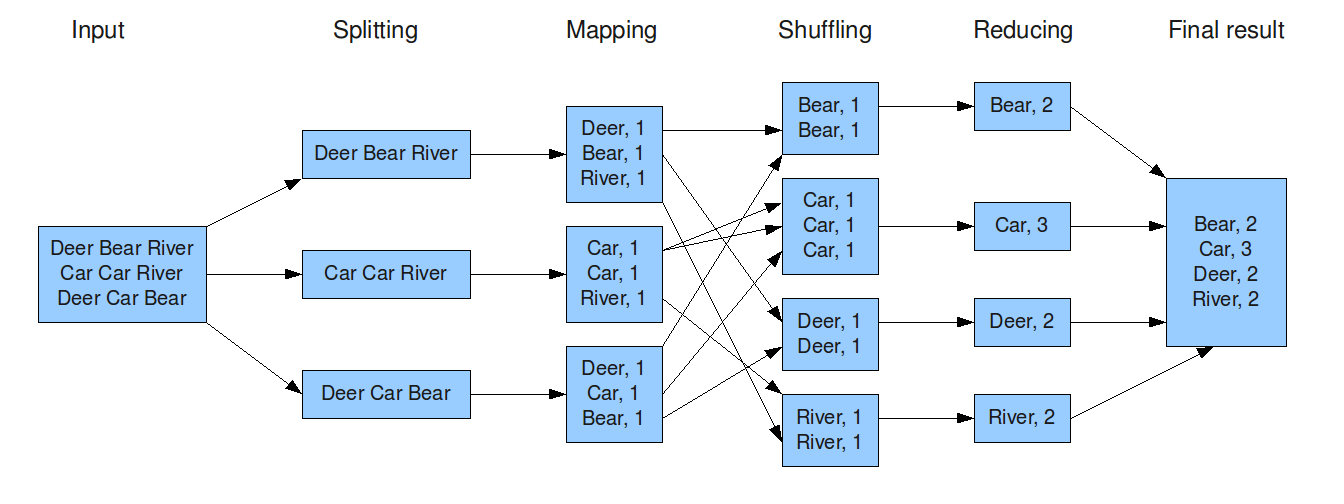
\includegraphics[width=\textwidth]{resources/img/mapreduce.png}
\caption{The overall MapReduce word count process\cite{mapreduce_img}}
%https://www.todaysoftmag.com/article/1358/hadoop-mapreduce-deep-diving-and-tuning
\label{img:mapreduce}
\end{figure}

Though the ease of implmenetation is very high and the technology is very appliccable to our platform, the algorithm has prooved to be comparatively slow. The reason for this is that before and after both the map and reduce phase the data has to be written to a distributed file system. Therefore though highly scalable, the approach suffers by slow disk writes\cite{mpareduce vs spark}. Finally, MapReduce works on large finite datasets. Therefore we need to manually preprocess stream data into batches in order for MapReduce to be applicable\cite{stream mapreduce}.

\subsubsection{Apache Spark (Streaming)}
Apache spark is an implementation of the Resiliant Distributed Dataset (RDD) paradigm. It entails a master node which partitions large datasets and distributes it among its slave nodes, along with instructions to be performed on individual data entries. Operations resemble the functions and methods of the Java Stream package \cite{java_stream}. 

Three sort of operations exist: narrow transformations, wide transformations and actions. \emph{Narrow transformations} are [item wise] operations that effect individual data entries and result in a new ([changed]) RDD, with the original RDD and target RDD partitioned [hetzelfde]. Examples of such functions are \emph{map} and \emph{filter}. Because these transformations are applied [item wise] and partitioning [are equal], many of these transformations can be performed consecutively without recalling the data to the master. \emph{Wide transformations} similarly are applied itemwize, but the target RDD may not be partitioned [gelijk] to the original RDD. An exapmle of such a transformation is \emph{groupByKey}. Since elements with  the same key must reside in the same partition, the RDD might require reshuffeling in order to continue. Finally,  Actions, such as \emph{collect} and \emph{count} do require all data to be recalled to the master and calculation is performed locally, resulting in a concrete return value (integer, list, etc.). RDD's [entail] an efficient distributed processing of large datasets, that is easy to write and read. However careful consideration must be given to the operations and execution chain in order to eliminate superfluous dataset redistribution.
%TODO refs

\begin{small}
\vspace{8px}\hrule
\begin{lstlisting}[
language=Java,
caption=MapReduce example of Figure \ref{img:mapreduce} in Spark RDD.,
captionpos=b, 
escapeinside={(*}{*)}, 
columns=flexible,
numbers=left,
tabsize=4,
breaklines=true,
label=list:mapreduce_spark-search
]
// assumes initial RDD with lines of words = lines
JavaRDD<String[]> wrdArr = 				lines.map(l->l.split(" "));
JavaRDD<String> words =					wrdArr.flatMap(arr -> Arrays.toList(arr));
JavaRDD<String, Integer> pairs =		words.mapToPair(x->(x,1));
JavaRDD<String, Integer> counts = 		pairs.reduceByKey((a,b) -> a+b);
Map<String, Integer> result =			counts.collectAsMap();(*\vspace{5px}\hrule*)
\end{lstlisting}
\end{small}

It is interesting to note that the MapReduce framework can easily be reproduced in Spark. this is achieved by calling the \emph{map} and \emph{reduceByKey} consequtively. To illustrate we implemented the MapReduce procedure of Figure \ref{img:mapreduce} in Apache Spark using Java in Listing \ref{list:mapreduce_spark-search}. Please note that the individual assignments of the RDD are not required. RDD-calls can be chained after one another, but intermediate assignments have been used to [illustrate] the steps taken. Also note that the first there steps are be performed fully parallized since they are all narrow transformations. Only line 5 (wide transformation) and 6 (action) require RDD redistribution.\cite{web:user_manual}
% ref e.g.: https://jaceklaskowski.gitbooks.io/mastering-apache-spark/spark-rdd-transformations.html

Additionally, the framework does not require disk writes (as MapReduce does). Instead, it runs distributed calculations in-memory, thereby vastly improving the overall calculation speed. This does however raises a reliability issue, because if a slave node fails it cannot recover it's state. This is resolved by the master by replicating the part of the dataset from the intermediate result it retained and distributing it among the remaining slave nodes. Because the [same] [chain] of transformations is applied to each individual entry in the dataset any new slave can continue calculations from that point.\cite{web:fault_tolerance}

Finally, Apache Spark suffers the same [problem] as MapReduce and is performed on finite datasets. Therefore streams need to be [collected] in batches in order to perform calculations. In fact Apache Spark [has] a library, Apache Spark Streaming\cite{web:spark_streaming}, which achieves [just that]. It batches input from streams on regular, pre-specified time intervals and supplies it to a Spark RDD environment. The time windows can be as small as a millisecond, therefore it is not formally real time, but does achieve near-real-time stream processing.

%TODO integration of communication techniques

\subsubsection{Apache Storm}
Apache Storm is a big data computing library especially designed for seperation of concerns. It performs distributed comuting by [seperting] the stages of computation. By breaking up the computation different stages can be distributed among machines and duplicated if need be. This is [performed] by three chief concepts. 
\begin{description}
\nospace
\item[Spouts:] nodes that introduce data in the [network],
\item[Bolts:] nodes that perform some computation or transformation on data, and
\item[Streams:] connect nodes to one another and allows data to be transferred.
\end{description}
The computation is regarded as a directed acyclical graph with bolts as vertices, spouts as [start vertices] and streams as edges.

Because data is emitted by spouts individually, Storm can achieve real-time processing of large amounts of data. By breaking up the compuations into multiple consequtive bolts, Storm allows computations to be spread over a cluster. Additionally Storm allows individual bolts to be replicated and distributed. This lateral distribution prevents the [occurrence] of bottlenecks in the network due to [expensive] singleton bolts.

Storm is especially [applicable] to our purpose since it was designed for microcomponents connected by streams. In [comparison] many micro-component platforms [focus] on components exposing services which are explicitly [called] by other services\cite{refs: spring, etc}. By employing Apache Storm we [recieve] both the distributed computation environment as the means of data distribution, simplifying our technology stack [check met kafka].

Conversely however, the built-in distrribution mechanism is completely internalized making integration with auxiliary processes difficult. Tasks such as data injection, platform monitoring and data extraction for processing or reporting by third-party stakeholders will require an exposing mechanism. Additionlly, Storm requires bolt connections to be expllicitly specified at startup. This [has] two implicated disadvatages. Firstly, we cannot update or reconfigure a single process without restarting the entire system. Considerations should therefore be made on when to update the system and when to delay rolling out an update. 

%TODO boven+onder samen nemen?
Secondly, the bolts are connected [one by one]. This is in contrast to [conventional] publish/subscribe communication platforms (such as Kafka\cite{web:kafka} and RabbidMQ\cite{web:rabbidmq} which decouple the producer and consumers and instead write and read to addressable communication channels called topics. Storm allows reading and listening on streams of a certain topic, but the connection still needs to be explicitly specified. This is cumbersome, but should be able to be overcome. Though [cumbersome], this also grants an advantage. With strong component bindings it should prove [more difficult] to [device] an invalid architecture due to small mistakes as mistypes and not updating all bindings on a refactor. 
%TODO iets over real time?

\subsection{Solution decision}
For distributed component platform we have chosen to build upon Apache Storm. The reason for this was primarily that Storm was conceived with this type of streaming micro-component application in mind. The spouts and bolts provide us with the [perfect] building blocks to design an iterative application with separation of concerns in mind, while the built-in stream mechanism provide the needs for a real-time distributed application. We will however need to account for the lack of [expose points] and the tedious process of specifying each and every bolt connection.

Though Storm [contains] the means for building a distributed accumulator process, we will not [use] it. Instead we will base our accumulator on Apache Spark Streaming. The reason for htis is that studies have shown Apache Spark to be 5 times faster than both MapReduce\cite{spark-vs-mapreduce} and Storm\cite{spark-vs-storm}. Spark does however have a larger latency, due to collecting batches of data instead of processing them real-time. This however should not cause a significant problem since our envisioned use case is for timed analysis jobs on very large amounts of input data, in order to detect or visualise collective tendencies of the system under investigation.

To facilitate external communication of the platform we will employ Apache Kafka. The reason for this is its speed and greater scalability. Additionally, but to a a smaller degree, [we chose it] because of Kafka's ability to multicast messages. This will allow multiple auxiliary processes to listen in on the proceedings of the platform. With our choice for Kafka comes another benefit, as the Spark Streaming library contains adapters for Kafka allowing direct connection to it. Therefore we can simply emit data to a Kafka topic and connect a Spark Streaming process to it. The [great] [incumbrance], being the lack of topic-level order guarentee, is not of grave [importance], because of the before mentioned [fix]. The hindrence cna be overcome by including timestamps or sequence numbers in the messages. Moreover, the Spark calculations most likely will not require order retention. The reaseon for htis is that most computations will consist of a \emph{reduce} step, which requires the reduction operation to be both associative and commutative\cite{ass-comm}. Therefore the message order is of no importance.

\section{Design}
We will adapt these technolgies by composing them using adapters and abstracting the solutions. By abstracting the technologies we shield the internal implementation details, simplifying [building] by the user. We will [supply] the user with some scaffoldings for bolts [intended for] different types of data flows and reductions. Additionally, on some [points] these solutions were abstract since they were intended for many [unforseen] usages. Since our [application] features some commonalities which were considered variations when designing the original technologies, we can implement some functions which were intentionally left unimplmeented originally. This will reduce the [implementatory] effort required, again simplifying usage of the platform.

\subsection{Micro-service architecture}
\subsection{Scaffolds for micro-services}
Distributor?
\section{Discussion}




%architecture
%	model reification
%what components needed
%	featuremodel
%	requirements
%which candidates
%benchmarking
%desicions
